%===================================
%===================================
%===================================
\setchapterpreamble[u]{\margintoc}
\chapter{SolarMED pilot plant}
\labch{solarmed:facility}

\glsresetall % Reset glossary entries

\tldrbox{The \gls{medLabel} pilot plant at \gls{psaLabel} is one of the first
demonstration plants of solar-powered desalination in the world and one of the
first facilities at \gls{psaLabel}. Over the years it has followed the evolution
of thermal desalination: from the seek for high-temperature, high-efficiency
complex systems (\glspl{tvcLabel}, \glspl{deahpLabel}) to the realization of
preferable simpler, lower-temperature systems. Today, it operates as a
\gls{medLabel} plant powered by a flat-plate collector solar field and a
two-tank thermal storage system, with water as the heat transfer fluid. This
chapter describes the main components of the facility, focusing on the
\gls{medLabel} plant, its particularities, instrumentation, and specifications.}

At the end of the 1980s, CIEMAT (Centro de Investigaciones Energéticas,
Medioambientales y Tecnológicas, Spain) and DLR (German Aerospace Center,
Germany) joined efforts to develop an advanced desalination system powered by
solar thermal energy and coupled to a \gls{tvcLabel}. This initiative, known as
the Solar Thermal Desalination (STD) Project
(1987--1994)~\sidecite{gregorzewski_solar_1991}, sought to demonstrate the
feasibility of coupling large-scale seawater desalination with solar energy.
During the first phase, a pilot plant was built at the \gls{psaLabel}, combining
a \gls{medLabel} unit with a parabolic-trough solar field and thermal oil
storage. The system operated with synthetic oil heated to drive steam
generation, reaching promising efficiencies and demonstrating high reliability.
However, the setup was complex and operated at relatively high temperatures,
requiring precise control and maintenance~\sidecite{milow_advanced_1997}.

In the second phase of the STD Project~\cite{milow_advanced_1997}, researchers
focused on improving energy efficiency and reducing consumption through system
integration. A \gls{deahpLabel} (LiBr-H$_2$O) was coupled to the \gls{medLabel}
unit, significantly lowering thermal demand and increasing performance ratios.
While these advancements confirmed the technical potential of solar-powered
desalination, they also highlighted the challenges of operating
high-temperature, oil-based systems. This realization guided subsequent efforts
toward simpler and more robust configurations.

A decade later, the AQUASOL
I~\sidecite{alarcon-padilla_application_2007,blanco_aquasol_2011} project built upon
this experience by shifting to lower-temperature and more practical designs. The
parabolic-trough field was replaced with a 500~m$^2$ stationary compound
parabolic collector (CPC) field using liquid water as the heat transfer fluid
and with a direct connection to the \gls{medLabel}. It included two small tanks
to attenuate fluctuations in thermal energy availability. The system could
operate in solar, fossil, or hybrid modes, offering greater flexibility and
easier operation. This transition marked a decisive move from complex,
high-temperature solar technologies toward simpler, water-based systems, better
suited for reliable and cost-effective desalination under real-world conditions.

In its current configuration, result of the AQUASOL-II
project~\sidecite{ampuno_modeling_2018,chorak_experimental_2017}, the
\gls{solarmedLabel} system consists of an \gls{medLabel} plant powered by a
flat-plate solar collector field coupled to a two-tank thermal energy storage
system (larger than previously), as shown in \reffig{intro:pilot-plants}. The
main components are interconnected as illustrated in
\reffig{solarmed:process-diagram}: a flat-plate collector field serving as the
heat source, a pressurized hot-water two-tank storage system, and an
\gls{medLabel} unit that utilizes this thermal energy to separate seawater into
freshwater and brine. The solar field and the storage circuit are thermally
coupled through a heat exchanger. Two subsystems can be distinguished: the
\fullgls{sftsLabel}, responsible for collecting and storing solar energy, and
the thermal load, which in this case corresponds to the \gls{medLabel} plant
performing the separation process (separation subsystem).

\begin{figure*}[h!]
	\includegraphics[]{SolarMED-process-diagram.png}
	\caption{\gls{solarmedLabel} process diagram}
	\labfig{solarmed:process-diagram}
\end{figure*}


% \section{Heat generation and storage subsystem}
% \labsec{solarmed:facility:sfts}

% Two pressurized water tanks coupled to a solar field composed of static flat
% plate collectors.


%================================
\section{Solar field}
\labsec{solarmed:facility:solar_field}


The AQUASOL-II solar field\sidenote{See \reffig{solarmed:process-diagram} -
\textit{Solar field}} consists of 60 static collector modules (Wagner LBM
10HTF model) with a total aperture area of 606 m$^2$, connected to a 40 m$^3$
thermal storage system through a heat exchanger\sidenote{Depicted in
\reffig{solarmed:facility:sfts}~(a)}. The solar field is arranged in
a small loop (Loop 1) with 4 collector modules connected in parallel, and four
larger loops (Loops 2--5), each composed of 14 collector modules (each loop
consists of two rows connected in series, and each row is formed by 7 collector
modules in parallel). All flat-plate collectors are oriented south and tilted
35° with respect to the horizontal plane~\sidecite{roca_modelo_2024}.

Each collector module is composed of five individual collectors through which
water circulates as the heat transfer fluid via a zigzag-shaped absorber tube.
As water moves across the tube, it absorbs solar radiation, increasing its
temperature before exiting the collector. Recently, the solar field has been
equipped with movable flat mirrors installed south of each collector row. These
mirrors automatically track the Sun and reflect direct solar radiation onto the
collectors, thereby increasing the solar irradiance incident on
them\sidenote{Even though this addition was performed recently and not
considered in this research work}. The design of the solar field allows
independent operation of each loop through its own valves and pumping system.
Each loop is connected to an individual heat exchanger, providing flexibility to
couple different loads according to experimental requirements.

% The solar field is basically a converter of electrical to thermal energy
% conditioned to the availability of solar irradiance. It has a total aperture
% area of 606 m$^2$ and can generate a maximum thermal power of 323 kW$_{th}$
% with a 1000 W/m$^2$ solar irradiance. It is composed of 4 loops each with 2
% rows of collectors... 

% The parameters of this facility are the shown in \reftab{solarmed:solar-field:parameters}.

% The parameters of this facility are the collector aperture ($A_c\,(m^2)$),
% number of parallel collectors in each loop, number of serial connections of
% collectors rows ($n_s$), number of parallel tubes in each collector ($n_t$) and
% the length of the collector inner tube ($L_t$). Their values are shown in
% \reftab{}.

% \begin{table}[H]
% \centering
% \caption{Nomenclature.}
% \labtab{solarmed:solar-field:parameters}
% \begin{tabular}{ll}
% \hline
% Name & Definition \\ \hline
% $A_c$ & Surface area of a collector (2.02 $\mathrm{m^2}$) \\
% $n_s$ & Number of serial connections of collectors rows ()
% \hline
% \end{tabular}
% \end{table}

%================================
\section{Thermal storage}
\labsec{solarmed:facility:thermal_storage}

% Imagen del campo solar
\begin{figure*}
    \centering
    \subfloat[\centering Solar field]{{\includegraphics[width=0.55\linewidth]{solarmed-solar-field.jpg}}}%
    \hspace{0.01\linewidth}
    \subfloat[\centering Thermal storage]{{\includegraphics[width=0.413\linewidth]{solarmed-thermal-storage.jpg}}}%
    \caption[]{Heat generation and storage subsystem facilities}
    \labfig{solarmed:facility:sfts}
\end{figure*}


% Imagen del almacenamiento

The thermal storage system\sidenote{See \reffig{solarmed:process-diagram} -
\textit{Thermal storage}} consists on a two-tank system. It has a total capacity
of 40 m$^3$ (depicted in \reffig{solarmed:facility:sfts}~(b)). The
system is based on the design principles outlined by Duffie and
Beckman~\sidecite{duffie_energy_2013}, and consists of two thermally insulated
tanks: a hot tank (the red tank in the diagram) operating at a higher
temperature and a cold tank (blue tank in the diagram), each serving distinct
roles in the thermal cycle (\ie ensure thermal stratification). In normal
operation, heat is extracted from the bottom of the cold tank, and after being
heated, it is injected into the top of the hot tank. The load extracts heat from
the top of the hot tank, and returns it to the bottom of the cold tank,
completing the cycle. The tanks are connected from top of the cold tank to the
bottom of the hot tank, allowing for recirculation of the fluid between the two
tanks.

%  One of the tanks
% (the red tank in the diagram) operates at a higher temperature, receiving heat
% from the energy source and delivering it to the load. The return flow from the
% load enters the bottom of the cold tank (blue tank in the diagram) before
% circulating back to the hot tank, where it absorbs heat from the source.


\section{\glsentrylong{medLabel}}
\labsec{solarmed:facility:med}

To understand the \glsentryfull{medLabel} process, it is useful to first
describe the operation of a single-effect distillation unit. Such a system
mainly consists of an evaporator and a condenser. In the evaporator, an external
heat source (typically hot water or steam from a boiler or power plant)
transfers energy to seawater sprayed over a tube bundle, forming a thin film
that partially evaporates. The generated vapor passes through a demister, which
prevents salt droplets from being carried over, and then condenses in the
condenser by transferring its latent heat to the seawater flowing inside the
tubes. This process yields two products: the distillate (condensed vapor) and
the brine (concentrated saline water). 

\begin{marginfigure}[-6.5cm]
	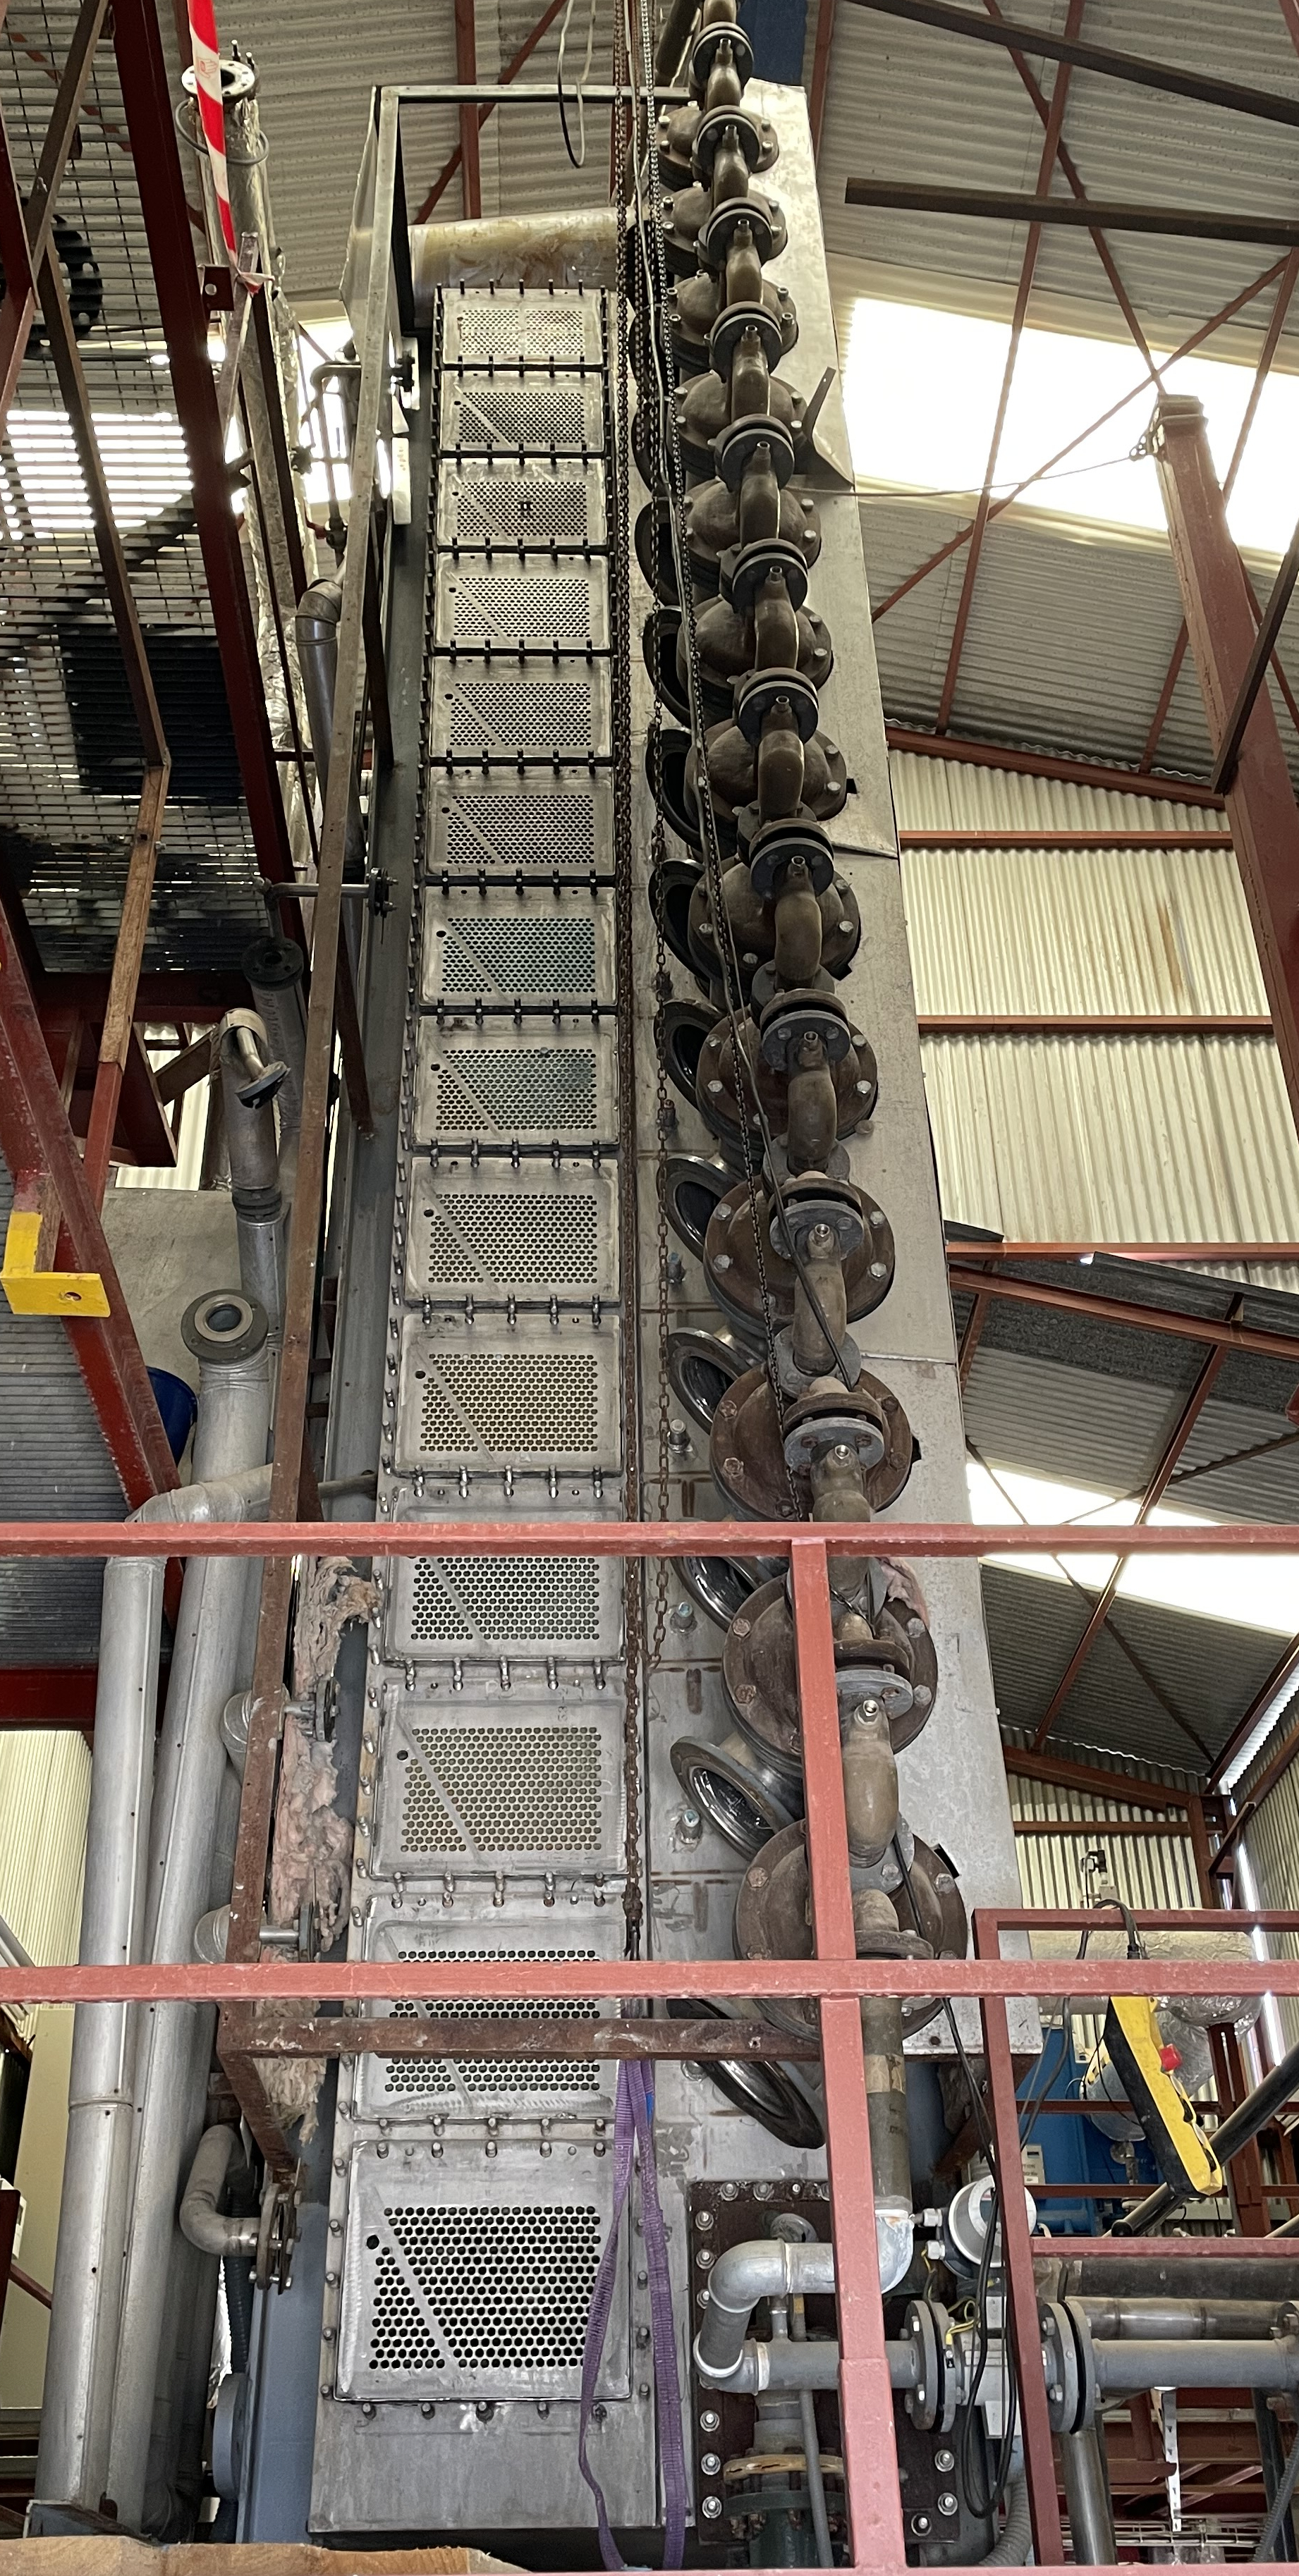
\includegraphics[width=.8\textwidth]{solarmed-facility-med.jpg}
	\caption{\gls{medLabel} plant at \gls{psaLabel} with open effects for maintenance}
	\labfig{solarmed:facility:med}
\end{marginfigure}


The condenser's cooling water removes the excess heat not used for evaporation,
and this water is discharged back to the sea. Since a single-effect unit has low
efficiency, multiple stages are connected in series in an \gls{medLabel} plant.
In this configuration, the vapor produced in one stage serves as the heat source
for the next, operating at progressively lower temperatures and pressures. Thus,
evaporation and condensation occur simultaneously in each effect, requiring only
one external heat source. The vapor condensed within all stages contributes to
the total distillate production, while the final stage's condenser preheats the
incoming seawater. Finally, the concentrated brine is
discharged~\sidecite{palenzuela_concentrating_2015}.

The experimental \gls{medLabel} plant at \gls{psaLabel} is a 14 effect,
vertically stacked, forward-feed plant initially built to use low-pressure
saturated steam as heat source (70~$^\circ$C, 0.31~bar) for the first effect
and, as mentioned, later replaced to use hot water. An image of the facility in
its current state can be seen in \reffig{solarmed:facility:med}. It has been
operated in different experimental campaigns and configurations robustly for
more than three decades. A summary of its main specifications
is shown at \reftab{solarmed:facility:specifications}.

% \reffig{solarmed:tests-calendar} shows the operation history of the plant (starting from 2009)

The first campaign from 2009 to 2012 is a comprehensive campaign covering the
operating range of the plant and described in
Palenzuela~\etal~\sidecite{palenzuela_experimental_2016}. Within the research
work presented in this thesis, a second experimental campaign took place between
2021 and 2025, in order to validate a standardization methodology proposal and
experimentally characterize the behavior of the system at higher temperatures
(see \refsec{solarmed:std:results}). It is not as extensive as the first one but
extends the operation range of the heat source temperature. In total, the
experimental data spans 6 years of operation and make available 549 operation
points with the range per variable shown in
\reftab{solarmed:modelling:med-data-range}\sidenote[][*-5]{Each experimental campaign
requires a significant number of test days due to the large number of target
operating points. Achieving a valid steady state takes approximately 20--30
minutes, not including the transition time between operating points. On a good
day, 3--4 stable operating points can be reached; on a bad day, due to for
example unfavorable environmental conditions, none may be achieved. This makes
the experimental campaigns complex and extensive, making it highly suitable for
extensive automation}.

Some particularities of this system are explained hereinafter:

\begin{itemize}
    \item As an energy efficiency measure, the plant is equipped with 13
    preheaters, which using a fraction of the vapor generated in the effects,
    preheat the feedwater before entering the first effect. The fourteenth
    ``preheater'' would be the condeser.
    
    \item As mentioned, the external heat source driving the process, is hot
    water from a thermal storage system. Water is drawn from one of the tanks
    and mixed with the water at the outlet of the first effect through a
    three-way valve (See \reffig{solarmed:process-diagram} - \textit{Three-way
    valve}), allowing independent regulation of flow and temperature.
    
    \item The inland location of this experimental plant is another
    particularity of the system. A fixed amount of seawater (30 m$^3$), stored
    in a reservoir, is available to be used in the process and replenished as
    needed. The effluents from the plant are mixed in a different reservoir (5
    m$^3$), and returned to the feed in a close loop operation. Because water
    exits the process at a higher temperature than when it enters, this type of
    operation implies an ever-increasing heat sink temperature. A wet cooling
    tower, installed between the two reservoirs, is used to mitigate this
    effect.

    \item The previous particularity leads to a significant variation in the
    inlet water temperature from day to day and also within the same day
    depending on the operation conditions. To ensure the stability of the
    condenser (i.e. a constant vapor pressure and outlet cooling water
    temperature), the cooling flow rate is regulated. This allows to have a
    stable system representative of a real plant operating under normal
    conditions. However, this can lead to variable electrical consumption of the
    cooling pump.

    \item The vacuum system of the plant is based on two hydro-ejectors and a
    pump. The pump is operated always at fixed speed and its electrical
    consumption has been characterized with measurements under various
    conditions as being near-constant and independent of the operation
    conditions. Its associated nominal power is 5 kW$_e$.

    \item The salinity of the feedwater is checked before every test measuring
    its conductivity with a conductivity meter (see
    \reftab{solarmed:facility:instrumentation}).

    % \item The distillate conductivity is measured every few tests in order to validate the proper operation of the plant (demisters, leakages, etc). The measurement of this variable is not considered necessary for each operating point, since a small variation in the order of 0.05 to 0.3 g/kg has been observed and therefore not deemed to have a significant effect on the results.
    % \item Brine and distillate extraction are controlled by keeping its respective levels constant by means of feed frequency regulation of the respective pumps. 
\end{itemize}


\begin{margintable}[*-25]
    \caption{\gls{medLabel} plant at \gls{psaLabel} specifications and nominal operating conditions}
    \labtab{solarmed:facility:specifications}
    \resizebox{\linewidth}{!}{%
	\begin{tabular}{@{}rl@{}}
	\toprule
	\multicolumn{1}{r}{\textbf{Parameter}} & \multicolumn{1}{l}{\textbf{Value}} \\ \midrule
	Capacity                               & 72 m³/day                          \\
	Number of effects                      & 14                                 \\
	Feed type                              & Forward feed                       \\
	Physical arrangement                   & Vertically stacked                 \\
	Heat exchanger configuration           & 90/10 Cu-Ni HTE                    \\
	Heat source type                       & Hot water                          \\
	Vacuum system                          & Hydro-ejectors                     \\ \midrule
	Heat source flow rate                  & 12 L/s                             \\
	Feed water flow rate                   & 8 m³/h                             \\
	Brine rejection                        & 5 m³/h                             \\
	Distillate production                  & 3 m³/h                             \\
	Cooling flow rate at condenser         & 8-20 m³/h (10-25 $^{\circ}$C)               \\
	Thermal power consumption              & 190 kW                             \\
	Top Brine Temperature (TBT)            & 70 $^{\circ}$C                              \\
	Condenser temperature                  & 35 $^{\circ}$C                              \\ \midrule
	\multicolumn{1}{l}{}                   &                                    \\
	\multicolumn{1}{l}{}                   &                                    \\
	\multicolumn{1}{l}{}                   &                                    \\
	\multicolumn{1}{l}{}                   &                                   
	\end{tabular}
	}
\end{margintable}

\begin{margintable}[*-10]
    \caption{\gls{medLabel} plant available experimental data range.}
    \labtab{solarmed:modelling:med-data-range}
    \resizebox{\linewidth}{!}{%
    \begin{tabular}{rccl}
    \toprule
    \textbf{Variable} & $\mathbf{\underline{x}}$ & $\mathbf{\overline{x}}$ & \textbf{Unit} \\
    \midrule
    $q_{s}$      & 10.50 & 44.35 & m$^3$/h \\
    $T_{s,in}$   & 52.01 & 80.98 & $^\circ$C \\
    $q_{f}$      & 4.98  & 8.27  & m$^3$/h \\
    $T_{c,in}$   & 12.14 & 33.64 & $^\circ$C \\
    $T_{c,out}$  & 19.36 & 39.89 & $^\circ$C \\
    $q_{d}$      & 1.61  & 3.08  & m$^3$/h \\
    $T_{s,out}$  & 50.05 & 77.31 & $^\circ$C \\
    $q_{c}$      & 8.03  & 23.13 & m$^3$/h \\
    \bottomrule
    \end{tabular}
    }
\end{margintable}


The experimental facility is a complex system of considerable size for a pilot
plant. It includes over 100 variables, between inputs and monitored outputs. Its
instrumentation is shown in \reftab{solarmed:facility:instrumentation} and the
placement in the system can be seen in \reffig{solarmed:facility:pid}.
\gls{pt100Label} sensors are used to measure all liquid temperatures
(\texttt{TT01}..\texttt{TT05}), while a PT1000 sensor is used to measure the
ambient temperature (\texttt{TT06}). The pressure inside the first effect and
condenser (\texttt{PT01} and \texttt{PT02}, respectively) is measured by two
different pressure transducers which fundamentally differ in their measurement
range. To monitor the power consumption of the system, various subsystems have
been individually instrumented using a power meter
(\texttt{JT01}..\texttt{JT04}). Conductivity is measured using a portable
conductivity meter (\texttt{CT01}, \texttt{CT02}), to which a calibration is
periodically performed to convert conductivity to salinity. Flow rates
(\texttt{FT01}..\texttt{FT04}) are measured using different types of flowmeters
depending on the characteristics of the fluid being evaluated. Electromagnetic
flowmeters are used for conductive fluids, while vortex flowmeters are used for
non-conductive fluids. All sensors transmit a \mbox{4--20 mA} analog signal that
is converted to digital by \gls{adcLabel} converters. \glspl{vfdLabel} are used
to control all flow rates in the system: heat source, cooling, feed, brine and
distillate.

\begin{table*}[]
\caption{Characteristics of the instrumentation installed at MED-PSA unit ($^a$ value of the measured temperature in $^\circ$C, $^b$ of reading, $^c$ full scale).}
\labtab{solarmed:facility:instrumentation}
\resizebox{\linewidth}{!}{%
    \begin{tabular}{@{}ccccc@{}}
    \toprule
    \textbf{Measured variable} & \textbf{Instrument} & \textbf{Model} & \textbf{Range} & \textbf{Measurement uncertainty} \\ \midrule
    Water temperature, TT01$\ldots$TT0N & PT100 Class A & SEDEM OF112871 & 0 - 100$^\circ$C & $\pm$ 0.15 + 0.002$\cdot T^{a}$ \\
    Distillate flow rate, FT03 & Vortex flow meter & ABB TRIO-WIRL VT4 & 1.6 - 18 m$^3$/h & $\pm$ 0.75\% o.r.$^{b}$ \\
    Hot water flow rate, FT01 & Electromagnetic & \begin{tabular}[c]{@{}c@{}}Endress+Hauser \\ Proline Promag 50P\end{tabular} & 2.42 - 78.33 L/s & $\pm$ 0.5\% o.r. \\
    Feedwater flow rate, FT02 & Electromagnetic & \begin{tabular}[c]{@{}c@{}}Endress+Hauser \\ Proline Promag P 300\end{tabular} & 2.1 - 66 m$^3$/h & $\pm$ 0.5\% o.r. \\
    Ambient temperature, TT05 & PT1000 & - & -40 - 60 $^\circ$C & $\pm$ 0.15 + 0.002$\cdot T$ \\
    Pressure, PT01 & Pressure capacitive & \begin{tabular}[c]{@{}c@{}}Endress+Hauser\\ Cerabar T-PMC131\end{tabular} & 0 - 1 bar & $\pm$ 0.5\% FS$^{c}$ \\
    Pressure, PT02 & Piezoresistive sensor & WIKA S-10 & 0 - 0.6 bar & $\pm$ 0.5\% FS \\
    Level, LT01, LT02 & Magnetic level gauge & IGEMA NA7-50 & 0-750 mm & $\pm$ 5 mm \\
    Power, JT01$\ldots$JT04 & \begin{tabular}[c]{@{}c@{}}Power meter Class 1\\ IEC 62053-21\end{tabular} & Circutor CM31 & 0-7 kW & $\pm$1\% o.r. \\
    Conductivity, CT01$\ldots$CT02 & Conductivity meter & \begin{tabular}[c]{@{}c@{}}Prominent \\ Portamess 911\end{tabular} & 0.1$\mu$S/cm - 1000~mS/cm & \begin{tabular}[c]{@{}c@{}}$\pm$ 0.5\% o.r. < 500 mS/cm\\ $\pm$ 1\% o.r. $\geq$ 500 mS/cm\end{tabular} \\ \bottomrule
    \end{tabular}%
}
\end{table*}

\begin{figure}
    \raggedleft
    \includegraphics[width=\textwidth]{solarmed-std-pid.png}
    \caption{\gls{pYidLabel} representative of the \gls{medLabel}-\gls{psaLabel}
    plant with the installed instrumentation, \glspl{kpvLabel}, and implemented
    control loops (\texttt{ANSI/ISA 5.1-2022}).}
    \labfig{solarmed:facility:pid}
\end{figure}